%%%%%%%%%%%%%%%%%%%%%%%%%%%%%%%%%%%%%%%%%%%%%%%%%%%%%%%%%%%%%%%%%
% Contents: Typesetting Part of LaTeX2e Introduction
% $Id$
%%%%%%%%%%%%%%%%%%%%%%%%%%%%%%%%%%%%%%%%%%%%%%%%%%%%%%%%%%%%%%%%%
\chapter{Modelling}

\section{Modelling}
To model the road tracking, various essential issues have to be considered such as how to identify road crossing object(s), how to encode different tracking directions, how to design the deep reinforcement learning network to determine the next action, etc. Such issues will be illustrated and addressed in this section.

\subsection{Road Tracking:} 
Our research is based on the SYNTHIA-SEQS-05 database \cite{Ros2016TheSYNTHIA}. Video sequences were recorded and saved, from which one extracted front,  rear, left and right view road images around the car for both right and left steering cars. Each view covers a range of angle up to 100 degrees. As a result, a large number of simulated image frames were provided, each has a resolution of $760 \times 1,280 \times 3$ pixel. 

The images were taken in four different environments: clear
environment in spring, fog environment, rain environment and
heavy-rain environment.

In our study, we look at forward view road frames for a right steering car in all four environments. 

To differentiate the main objects on the road, specific colours were used, e.g., sky is grey, buildings are brown, roads are purple, side walks are blue and road markings are green. In other words, the purple and green colours refer to the allowed driving regions.  

More specifically, each view (image) can be divided into a safety zone and a danger zone. The safety zone is the zone that a car can keep moving to, as it is further away and it allows ample time to stop or slow down the car if necessary. The danger zone is the area that a car must stop if any objects are recognised. Such zones can be found in Fig. \ref{Fig:segmentation_regions}(e-k). 

How do we determined a safe zone or a danger zone? In each image of Fig. \label{Fig:segmentation_regions1}, a virtual triangle and trapezoid were drawn. The base of the triangle and trapezoid moves in the road direction, and the crossing lines can slope toward the tracking direction. The height of the triangle (and the trapezoid) is two thirds of the acquired image. The top one third of the trapezoid is the safety zone and the bottom two thirds is the danger zone. The shared point of the triangle and the trapezoid is called an anchor point. It denotes the road tracking direction. The anchor point can denote the direction by following the track centre. By drawing the virtual triangle in the trapezoid area is to specify three types of regions: left, right and centre. These regions can specify the direction of any crossing object. The car can, for instance, avoid an object crossing from the left side by moving to the right, if the space is empty there. If objects are identified from both sides in the danger zone, then the car has to stop.  

\subsection{Actions codes:} 
At any point, the following actions can be taken by a car: drive straight on, turn left or right, reverse and stop. In our work, we use a five-digit binary number to encode each action, see Table \ref{Table:Signs_codes}. The stop action is applied when the danger zone recognising object(s) in the way from both sides. 

When a crossing object is detected, it will change the action from that side with a ``0". For instance, the car is moving forward with action 01110, then an object appears in the danger zone from left, then the action becomes 00111. When another object appears from the right, the code will be 00110 and the car will stop. As long as there are no three consecutive 1's, the car has to stop.  We model all such cases as 00000 to reduce the number of coding values. Fig. \ref{Fig:segmentation} shows explanations for various coding cases.

The binary codes can be converted to desired equivalent codes. A standard conversion from the binary to decimal \cite{koren2001computer} is used. For instance, $(01110)_2=(14)_{10}$ and $(00111)_2=(7)_{10}$. The only exception here is the backward direction, where a negative sign (-) is added to refer to the reverse movement. It is worth mentioning that the reverse action can only be considered if the car is being out of the track. The road tracking actions with their suggested codes and descriptions are given in Table \ref{Table:Signs_codes}. The decimal codes are used in the regression layer of the proposed deep reinforcement learning network as will be explained later. They are referring to road tracking actions.

\begin{table}[!h]
	\centering
	\caption{The road tracking actions with their suggested codes and descriptions}
	\label{Table:Signs_codes}
	\begin{tabular}{|c|C{2cm}|C{2cm}|C{5cm}|}
		\hline
		\textbf{Action sign} & \textbf{Binary code} & \textbf{Equivalent decimal code} & \textbf{Description} \\ \hline
		\begin{minipage}{.075\textwidth}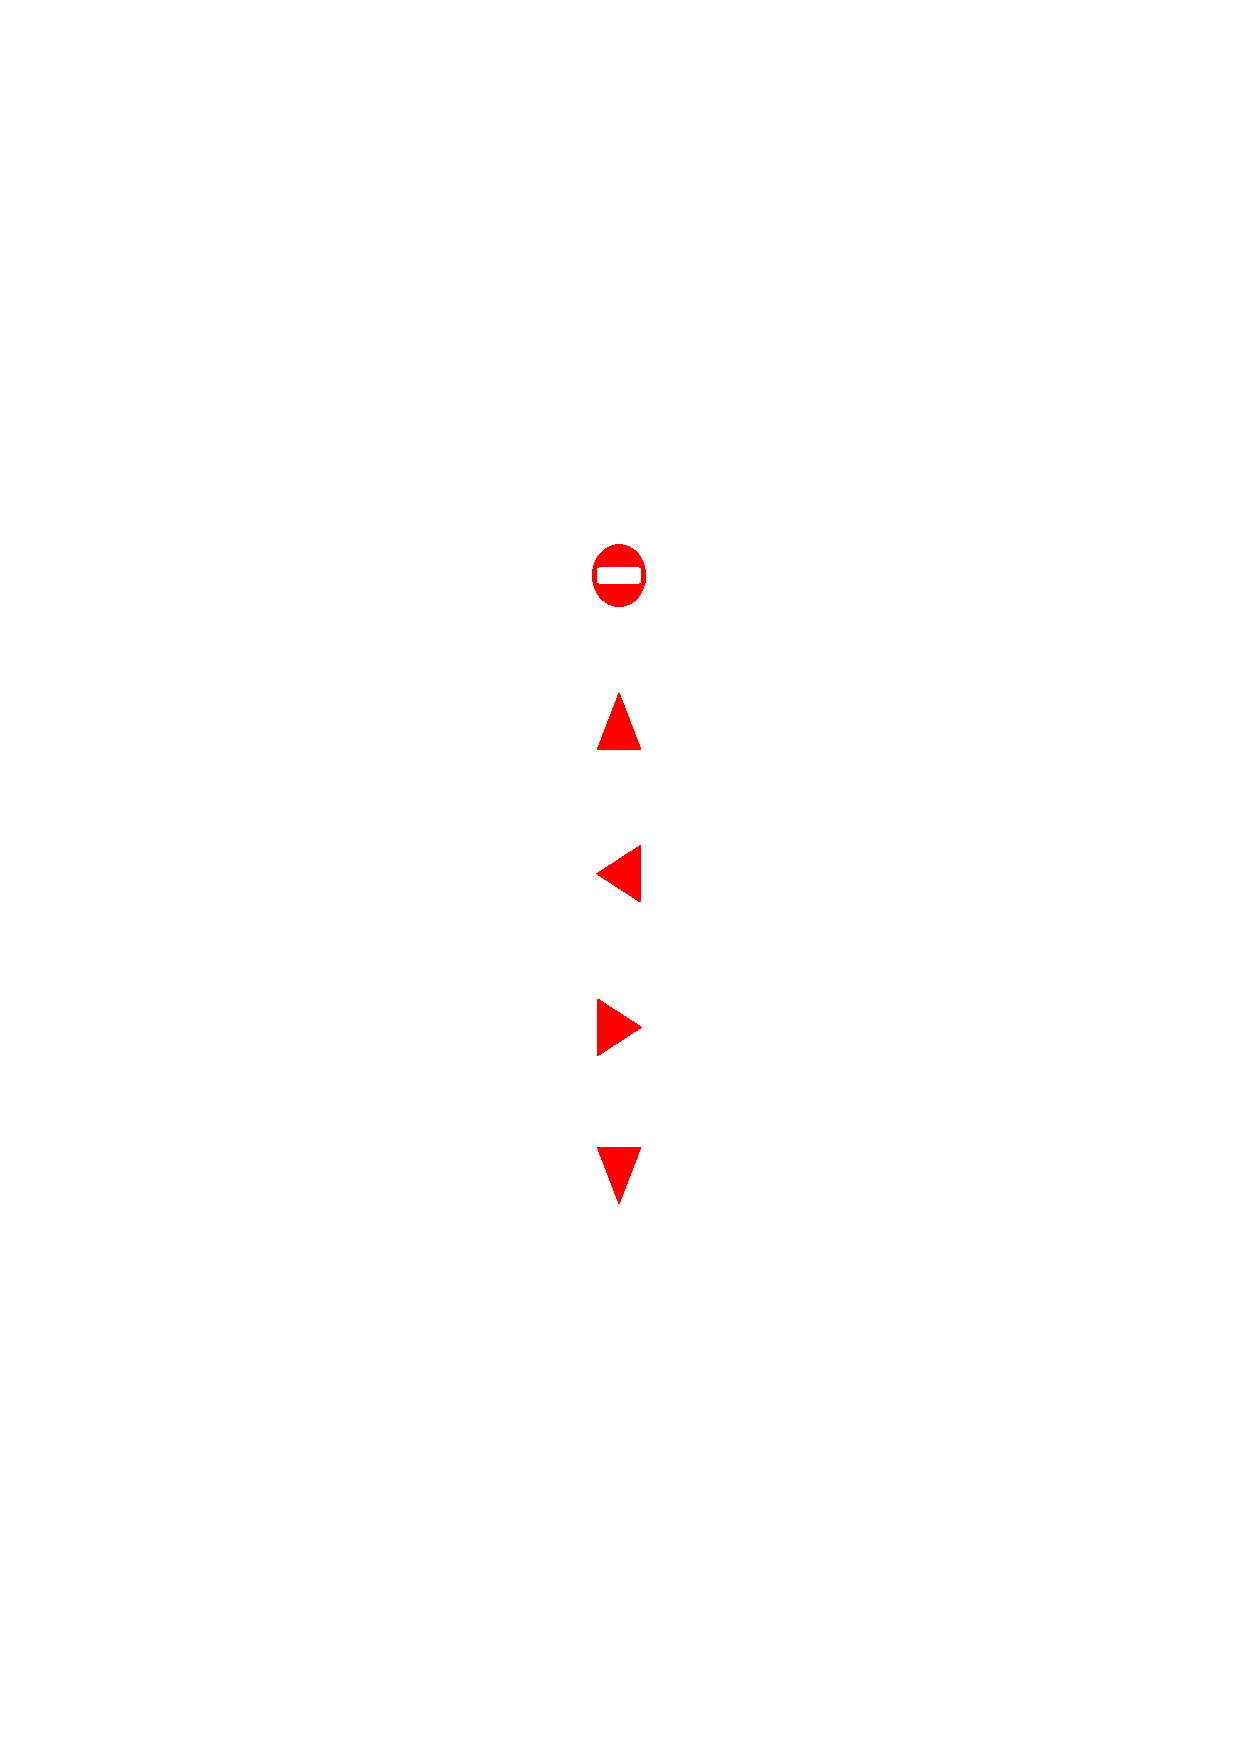
\includegraphics[scale=.5,trim=9.1cm 18.5cm 9.5cm 8cm,clip]{signs.pdf}\end{minipage}	& 0 0 0 0 0 & 0 & Stop (stop action because of crossing object(s)) \\ \hline
		\begin{minipage}{.075\textwidth}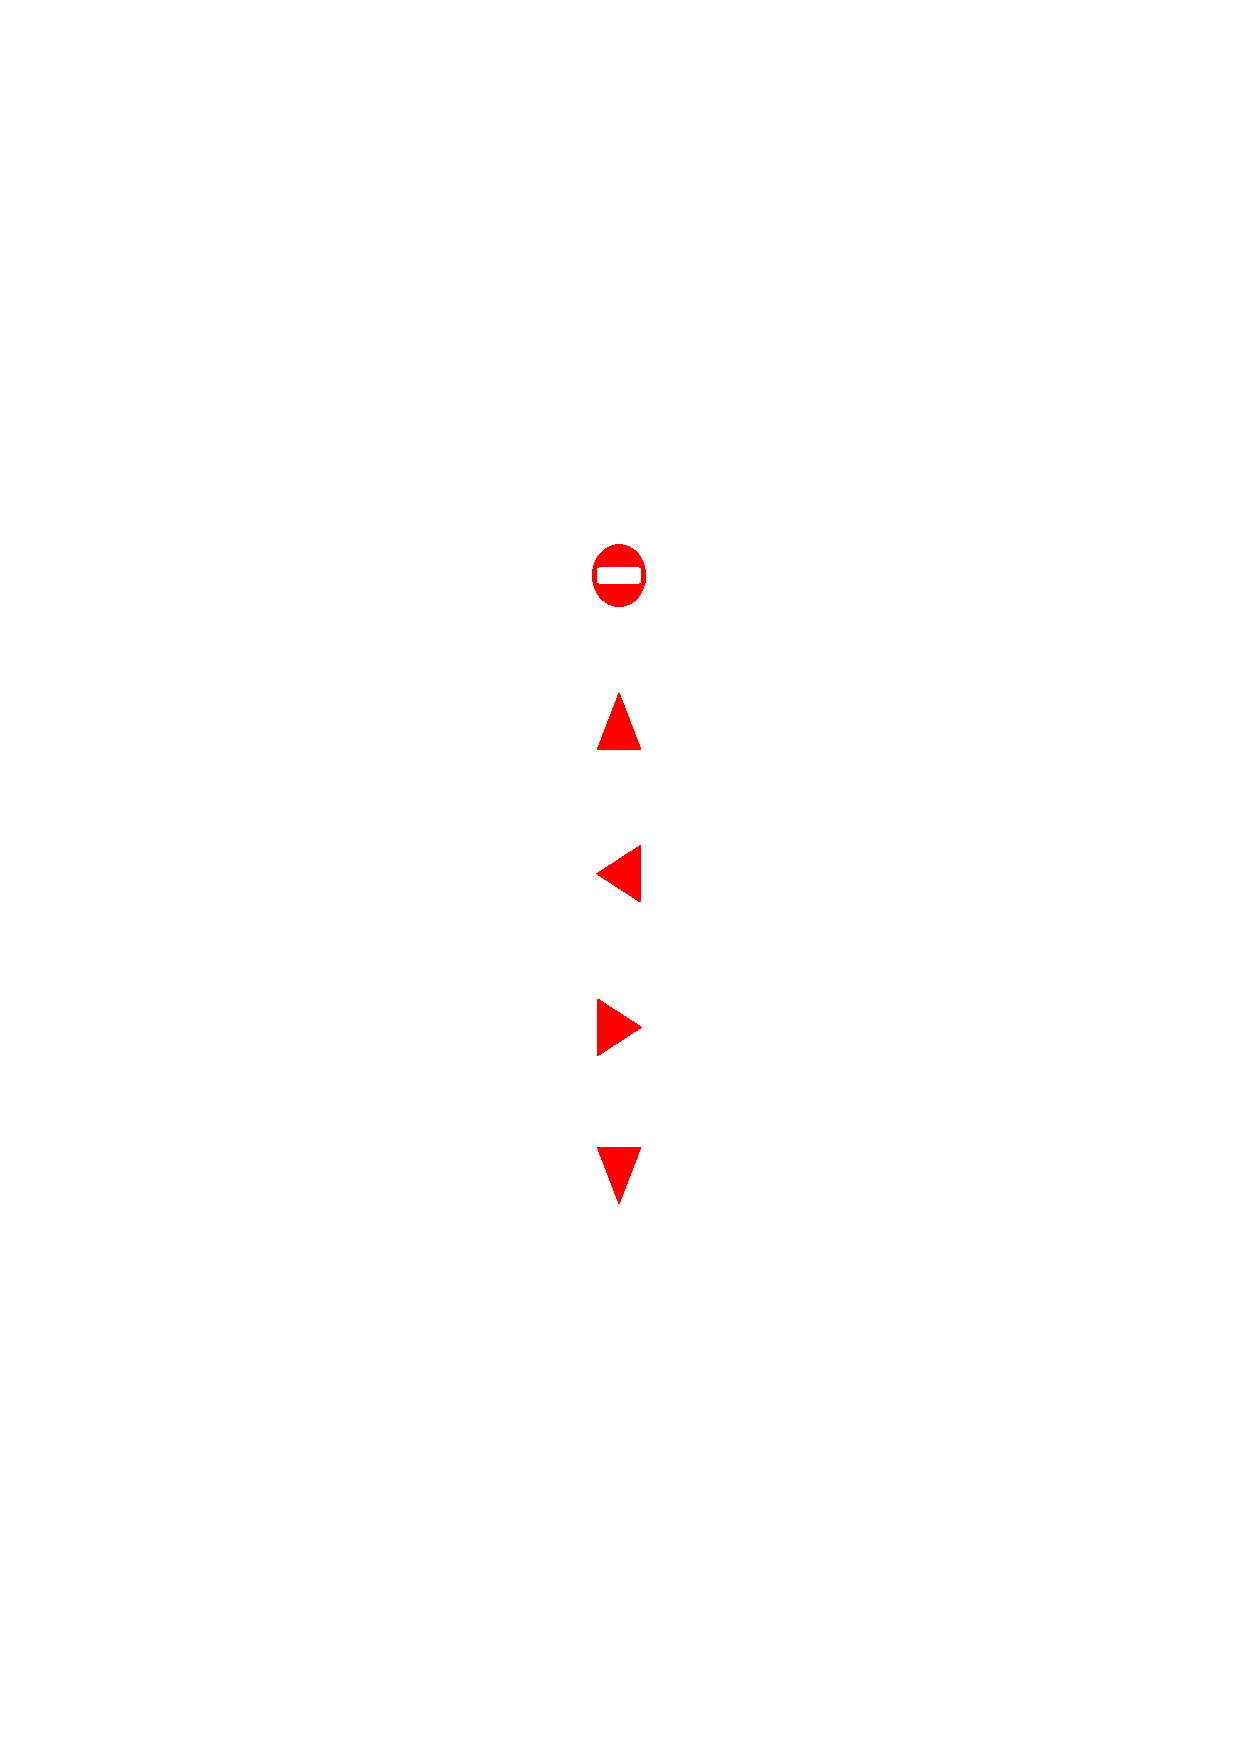
\includegraphics[scale=.5,trim=9.1cm 16cm 9.5cm 10.5cm,clip]{signs.pdf}\end{minipage}	& 0 1 1 1 0	& 14 & Move straight forward (follow the track to the forward direction) \\ \hline
		\begin{minipage}{.075\textwidth}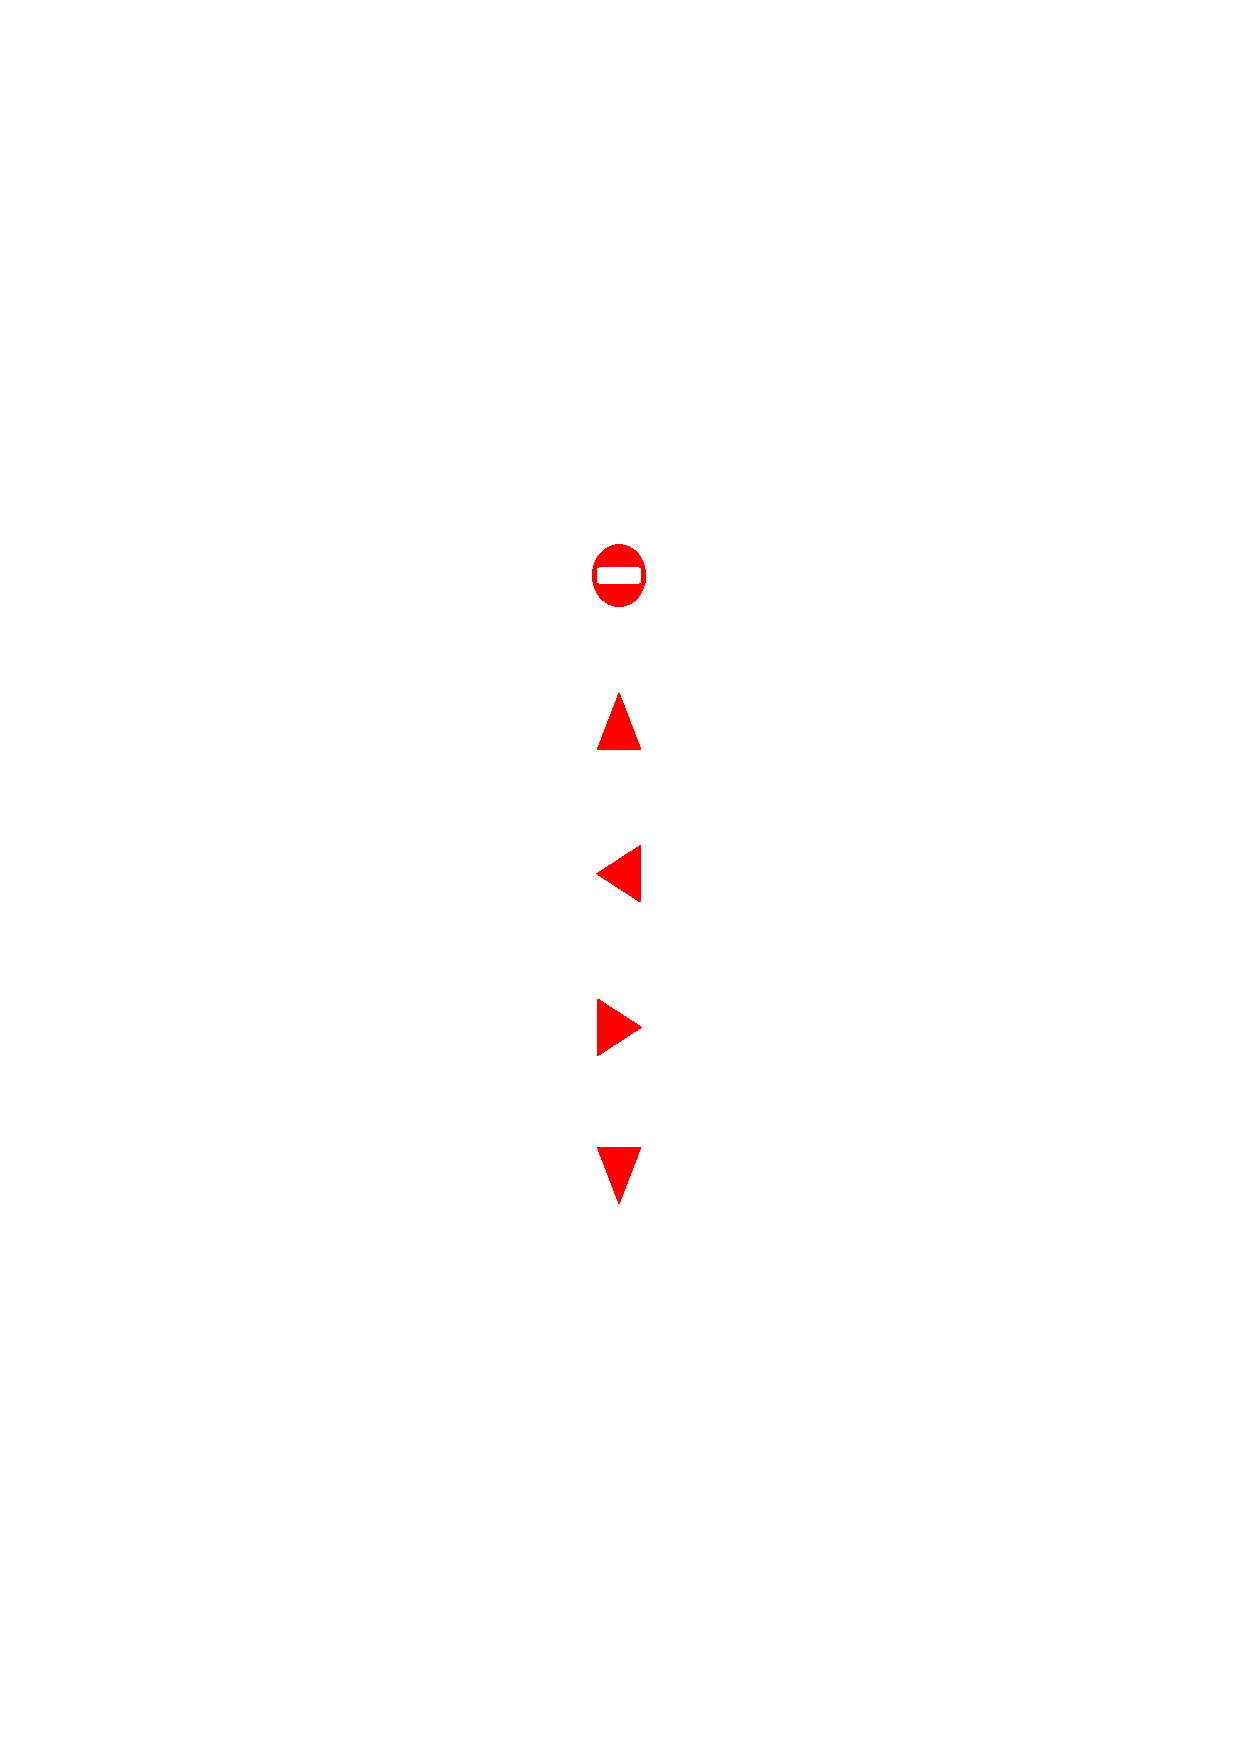
\includegraphics[scale=.5,trim=9.1cm 13.5cm 9.5cm 13cm,clip]{signs.pdf}\end{minipage}		& 1 1 1 0 0 & 28 & Move to the left (follow the track to the left direction) \\ \hline
		\begin{minipage}{.075\textwidth}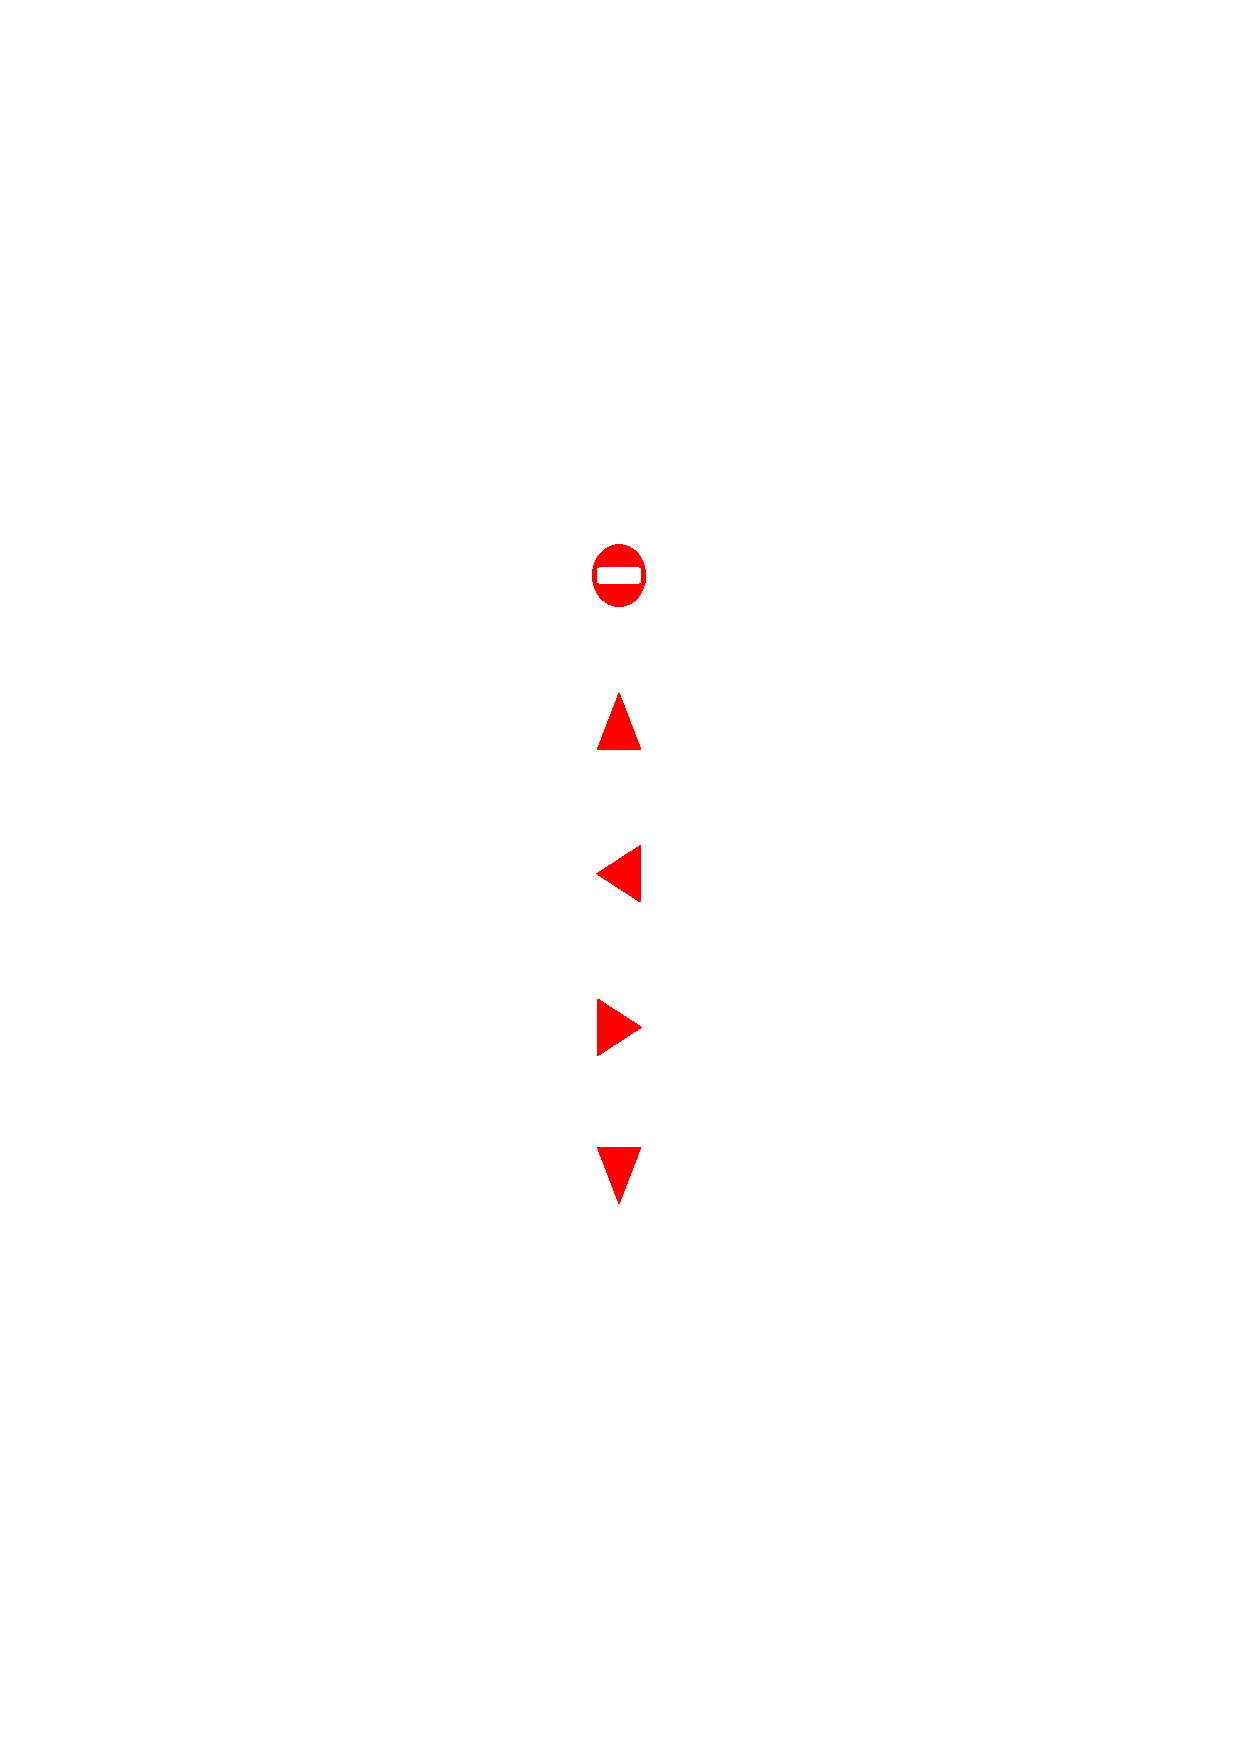
\includegraphics[scale=.5,trim=9.1cm 10.75cm 9.5cm 15.75cm,clip]{signs.pdf}\end{minipage}	& 0 0 1 1 1 & 7 & Move to the right (follow the track to the right direction) \\ \hline
		\begin{minipage}{.075\textwidth}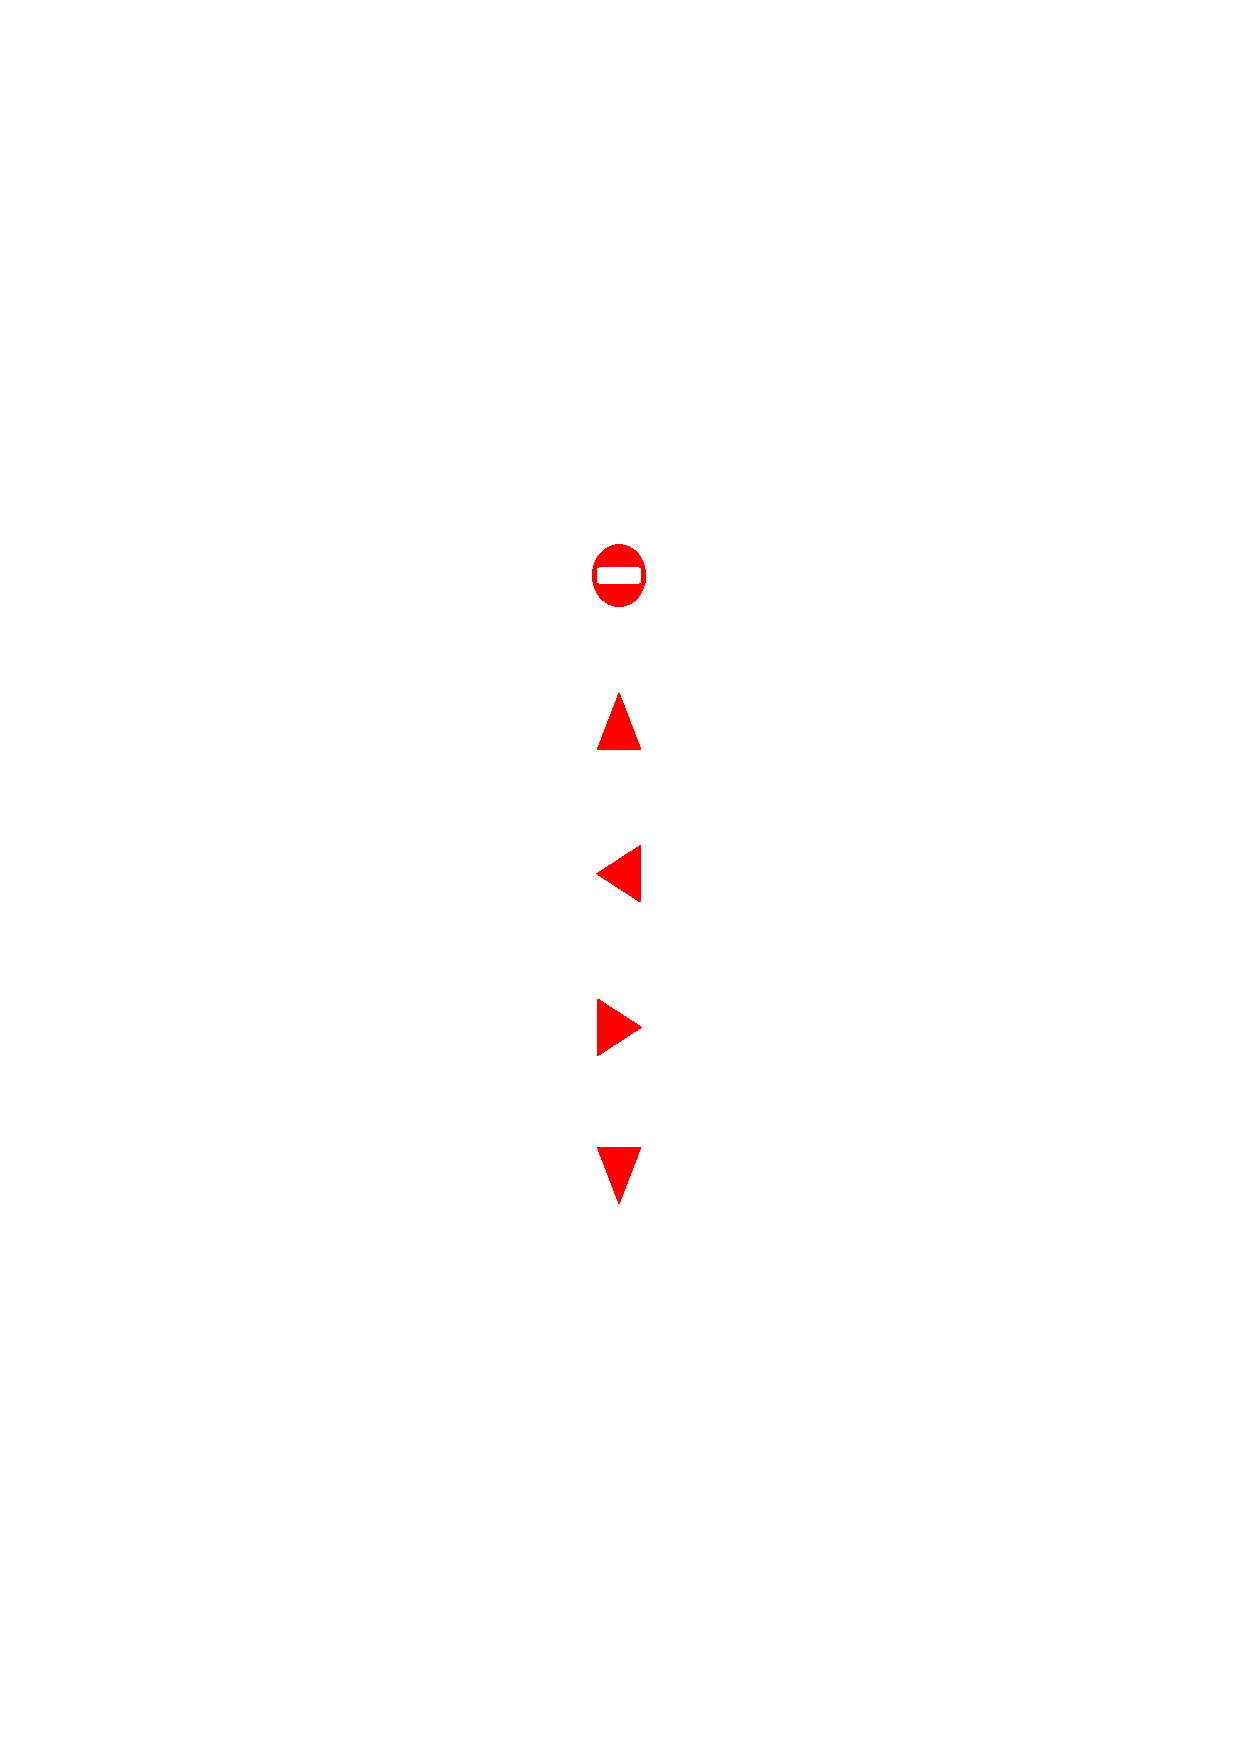
\includegraphics[scale=.5,trim=9.1cm 8.5cm 9.5cm 18cm,clip]{signs.pdf}\end{minipage} & 1 1 1 1 1 & -31 & Move backward (reverse moving to the back) \\ \hline
	\end{tabular}
\end{table}

\subsection{Policy search:} 
Principally, there are two essential types of reinforcement learning methods - policy search and value function. The first type refers to methods that consider searching for the optimal policy $\pi^*$. The second type refers to methods that consider investigating the optimal value-state function $V^*(s)$ \cite{Arulkumaran2017Deep}. In this work, the suggested DRL-RT network is based on the policy search. According to the MDP concept, the DRL-RT collects input images as current states $S_t$ and getting advantages from rewards $R$ to generate actions $A$, then the actions predict new states $S_{t+1}$. Consequently, the new states can be transitioned again in the inputs as current states. 

The essential equation of the policy search is demonstrated as:
\begin{equation}
\pi^*=\underset{\pi}{argmax}~\mathbb{E} [R\mid\pi]
\label{Eq:MDP}
\end{equation}
where $\pi$ is the policy and $\mathbb{E}$ is the expected return value \cite{arulkumaran2017brief}. In this work, the reward $R$ of the correct tracking is considered as (+1), whereas, the reward $R$ of the incorrect tracking is considered as (-1). Measuring the successful process of the road tracking will be based on obtaining as many positive rewards as possible. 

\subsection{Proposed DRL-RT:} 
An applicable deep reinforcement network named the DRL-RT is established for road tracking. It consists of eight layers: two convention layers, two Rectified Linear Unit (ReLU) layers, a pooling layer, a fully connected layer, a regression layer and a classification layer. The input is an image of a car facing view, and it is considered as a current state. The input image size has been reduced to $254 \times 427 \times 3$ pixels in order to speed up the deep learning processes. The first layer after the input is a convolution layer, it consists of 5 filters each of which has a filter size of $10 \times 10$ pixels. This layer is important to extract the main features of the input images. A ReLU layer is used in the second layer. It removes the negative values and maintain the positive values of the previous layer. The third layer is also a convolution layer, it consists of 5 filters each of which has a filter size of $5 \times 5$ pixels. It extracts more features from the input images. A ReLU layer is employed again in the fourth layer. This layer rectifies the negative values. It has empirically been found that using two convolution layers with two ReLU layers can well analyse the information before being compressed by applying the next layer. Then, a pooling layer of a maximum type is applied in the fifth layer, the filter size here is $3 \times 3$ pixels with a stride of 3 pixels. The sixth layer is a fully connected layer, it collects the outputs from the previous layer and produces a series of decimal code tracking values. A regression layer is the seventh layer. In this layer, a series of directional road tracking codes are generated. The successful codes in this layer produce positive rewards, whereas, unsuccessful codes generate negative rewards. The network should be propagated, forwarded and backwarded the information for updating the network weights, during the training stage till obtaining as many positive rewards as possible. Given the codes in the regression layer, it is the classification layer's task to generate a new action - one of the five as in Table \ref{Table:Signs_codes}. Fig. \ref{Fig:Deep_Reinf_Net} shows the proposed DRL-RT network.

\subsection{Theoretical concepts:} 
The theoretical concepts of the main analysis layers (convolution, ReLU, pooling and fully connected) in the DRL-RT network were stated in \cite{omar2018deep}.

In the first and third layers, the collected information will be converted to feature maps. The feature map is defined as a convoluted 2D image with a kernel of weights. The following general equation represents the operations in a convolution layer:
\begin{equation}
z_{u,v,c^{l}}= \text{\footnotesize $B_{c^{l}}+\sum_{i=-k_h^{l}}^{k_h^{l}}\sum_{j=-k_w^{l}}^{k_w^{l}}\sum_{c^{l-1}=1}^{C^{l-1}} W_{i+k_h^{l},j+k_w^{l},c^{l-1}}^{c^{l}} z_{u+i,v+j,c^{l-1}}$}
\label{eq:conv_layer}
\end{equation}
where $z_{u,v,c^{l}}$ is a convolution layer outcome, $(u,v)$ is the assigned pixel, $c^{l}$ is the channel number of the convolution layer,  $W_{i,j,c^{l-1}}^{c^{l}}$ is the components of the kernel weights,  $B_{c^{l}}$ is the channel bias of the convolution layer, $k_h^l$ and $k_w^l$ are respectively the height and width of the kernel weights of the convolution layer, $C$ is the number of channels and it is here equal to 3 as we are using three channels of coloured images, $l-1$ is the previous layer, and $l$ is the current layer (the convolution layer) \cite{simo2016learning}. 
% \marginpar{Does it mean that all the $k_w^l$ are the same for all layers?}. Answer is: no and I have mentioned previously that $l$ represents the current layer.
%Again, this layer analyses the input values and produces FTs' feature maps.

A ReLU transfer function is applied in the second and fourth layers. This function can provide non-linear calculation to the DRL-RT. The ReLU function maintains the positive values and discards the negative values of a previous layer. Equation \eqref{eq:relu_layer} is exploited for the ReLU transfer function:
\begin{equation}
o_{u,v,c^{l}}=f(z_{u,v,c^{l}})=\max(0,z_{u,v,c^{l}})
\label{eq:relu_layer}
\end{equation}
where $o_{u,v,c^{l}}$ is a ReLU layer outcome and $\max$ is the maximum operation \cite{krizhevsky2012imagenet}. 

A pooling layer is used in the fifth part of the DRL-RT. The pooling layer can reduce the sizes of the feature maps. It obtains the maximum values from the last ReLU layer. In general, the pooling layer can be applied according to the following equation:
\begin{equation}
q_{a^{l},b^{l},c}=\underset{0\leq a<p_h,0\leq b<p_w}{\max} o_{a^{l}\times p_h+a,~b^{l}\times p_w+b,~c}
\label{eq:pooling_layer}
\end{equation}
where $q_{a^{l},b^{l},c}$ is a pooling layer outcome, $0\leq a^{l} <p_h^{l}$, $p_h^{l}$ is the height of the resulting feature maps, $0\leq b^{l} <p_w^{l}$, $p_w^{l}$ is the width of the resulting feature maps, $0\leq c <C^{l}=C^{l-1}$, $p_h$ and $p_w$ are respectively the width and height of the feature map sub-areas that require pooling \cite{wu2017introduction}. 

Subsequently, the fully connected layer is used to match between the designed number of subjects and the data of the pooling layer. Equation (\ref{eq:fully_connect}) demonstrates the fully connected layer processes:
\begin{equation}
g_{r}=\text{\footnotesize $\sum_{a=1}^{m_1^{l-1}} \sum_{b=1}^{m_2^{l-1}} \sum_{c=1}^{m_3^{l-1}} W_{a,b,c,r}^{l}(\textit{\textbf{Q}}_{c})_{a,b}~, ~~~~~~~\forall 1 \leq r \leq m^{l}$}
\label{eq:fully_connect}
\end{equation}
where $g_{r}$ is a fully connected layer outcome, $m_1^{l-1}$ and $m_2^{l-1}$ are the width and height of a feature map in the previous layer (the pooling layer) respectively, $m_3^{l-1}$ is the number of produced feature maps in the pooling layer, $W_{a,b,c,r}^{l}$ is the connection weights between the fully connected layer and the pooling layer, $\textit{\textbf{Q}}_{c}$ are the pooling layer outputs, and $m^{l}$ is the number of designed subjects \cite{stutz2014neural}.

The computations of the regression layer in the suggested DRL-RT network are based on the Mean Squared Error (MSE). The main MSE equation is illustrated as:
\begin{equation}
MSE=\frac{1}{n} \sum_{r=1}^{n}(t_r-g_r)^2
\label{eq:fully_connect}
\end{equation}
where $n$ is the number of computed values and $t$ is the desired output values \cite{saugirouglu2009intelligent}. If the regression output values close to the desired code values, positive rewards are produced. Otherwise, negative rewards are generated. 

Finally, the classification layer translates the regression information into actions by converting the obtained values into their assigned classes.

The MDP has been applied to the DRL-RT by providing current road tracking as current states $S_t$ to the input layer, estimating tracking directions as actions $A$, considering correct and incorrect tracking actions as rewards $R$, and predicting next tracking movements as new states $S_{t+1}$. Then, the new state (or next tracking view) are transitioned as a current state to the DRL-RT input layer in order to produce a new state again.
\begin{table*}[!t]
	\centering
	\caption{Examples of the four employed environments}
	\label{Table:Environments_Examples}
	\begin{tabular}{|C{1cm}|c|C{13.5cm}|}
		\hline
		\textbf{Database no.} & \textbf{Environment} & \textbf{Examples} \\ \hline
		(1)	& Spring & \begin{minipage}{.9\textwidth}\includegraphics[scale=.8,trim=2cm 24.5cm 2cm 2.5cm,clip]{examples.pdf}\end{minipage} \\ \hline
		%			&&\\ \hline
		(2) & Fog	& \begin{minipage}{.9\textwidth}\includegraphics[scale=.8,trim=2cm 20.5cm 2cm 6.5cm,clip]{examples.pdf}\end{minipage} \\ \hline
		%			&&\\ \hline
		(3)	& Rain &  \begin{minipage}{.9\textwidth}\includegraphics[scale=.8,trim=2cm 16.5cm 2cm 10.5cm,clip]{examples.pdf}\end{minipage} \\ \hline
		%			&&\\ \hline
		(4)	& Heavy- rain & \begin{minipage}{.9\textwidth}\includegraphics[scale=.8,trim=2cm 12.5cm 2cm 14.3cm,clip]{examples.pdf}\end{minipage} \\ \hline
		%			&&\\ \hline
	\end{tabular}
\end{table*}
